% !TeX encoding = UTF-8

%===============================================================================
% Font options are:
%   plain (default), serif (uses Palladio), sans-serif (uses Paratype Sans)
%
% Layout options are:
%   article (default, no chapters), book (for longer texts, offers \chapter)
%   Changing this value between LaTeX runs may require deleting the .aux files
%
% Paragraph options are:
%   noparskip (default, no spacing between paragraphs), parskip (spaced)
%
% Language options are:
%   de (default), en
%   Changing this value between LaTeX runs may require deleting the .aux files
%
\documentclass[serif,article,noparskip,en]{agse-thesis}

% Global parameters, replace with actual values.
\newcommand{\thesisTitle}{Exploratory Analysis of Cultural Differences in Programming Language Communities}
% -> You may use \par (but not \\) to format the title. If you do so, you'll
%    need to manually set the 'pdftitle' attribute below.
\newcommand{\studentName}{Anton Rafael Wille}
%===============================================================================

\hypersetup{pdftitle={\thesisTitle}}
\hypersetup{pdfauthor={\studentName}}

\addbibresource{bibliography.bib}

\begin{document}

\coverpage[
    student/id=5093261,
    student/mail=anton.wille@fu-berlin.de,
    thesis/type=Bachelorarbeit,            % optional, default: Bachelorarbeit
    thesis/group={Arbeitsgruppe Software Engineering},
                                           % optional, default: AGSE
    thesis/advisor={Prof. Dr. Lutz Prechelt},           % optional
    thesis/examiner={Prof. Dr. Lutz Prechelt},
    thesis/examiner/2={Prof. Dr. Claudia Müller-Birn}, % optional
    thesis/date=\today,                    % optional, default: \today
   %title/size=\LARGE,      % set this value to overwrite automatic font size
   %abstract/separate       % toggle this to move the abstract to its own page
]
{ % Your abstract here:
    \noindent
    Taking a Grounded Theory (GT) approach to discussions on the QA-platform StackOverflow, this exploratory work aims
    to find, analyse and compare cultural characteristics in the communities forming around Perl, Python and Ruby,
    and contrast them wherever they diverge, with the idea that differences in design decisions, different contexts
    of practice, and distinct histories lead to different pronounciations in culture.
    During the exploratory process, multiple interesting directions of investigation were opened, with two main questions
    emerging: \textit{“Should there be one or multiple ways of doing things in a programming language?”},
    and \textit{“What does it mean to write idiomatic code?”}. The thesis offers some preliminary answers to these questions,
    insights into the character of these communities, and can hopefull serve as a springboard for future investigations.
}

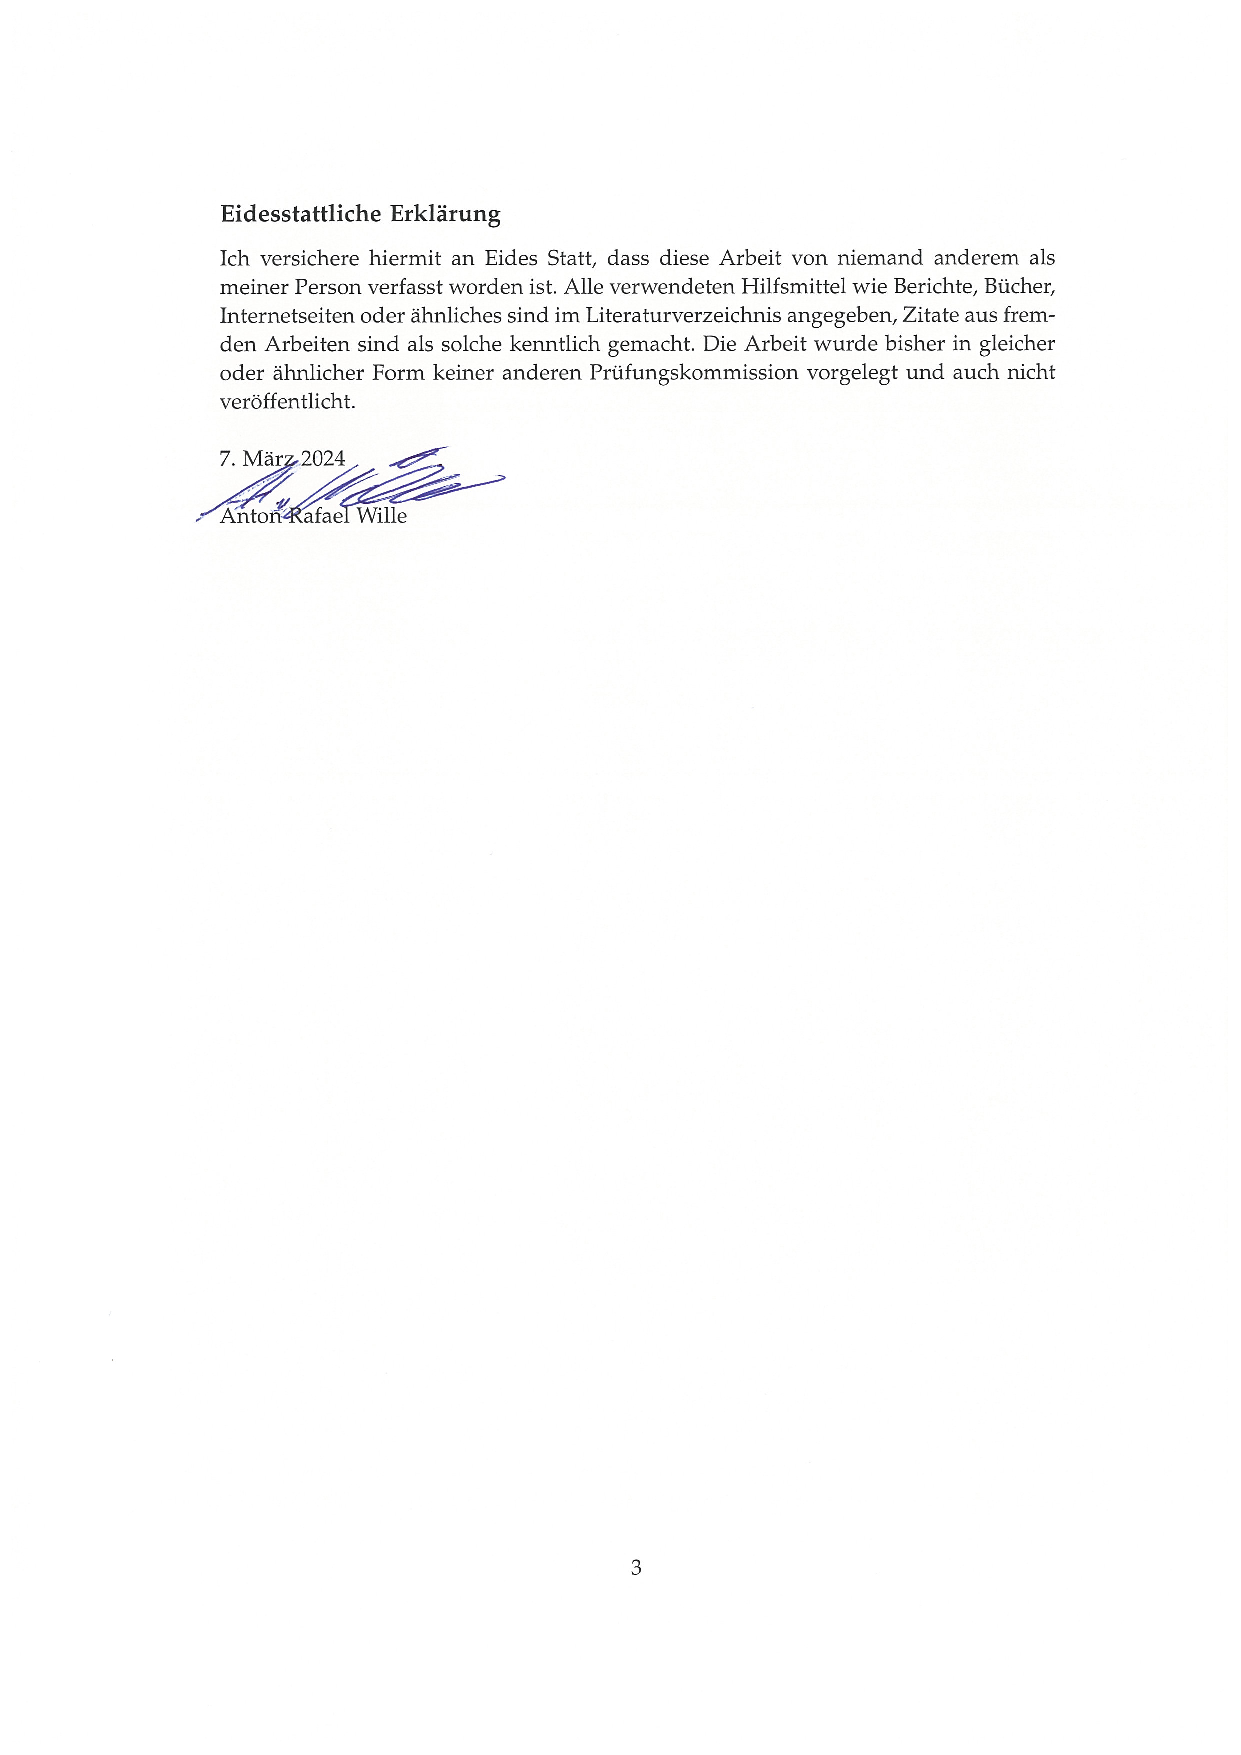
\includepdf[pages=-]{declaration.pdf}

\cleardoublepage

\tableofcontents

\cleardoublepage

\pagestyle{fancy}

% Actual content starts here

% !TeX encoding = UTF-8
\section{Introduction}

While much attention has been dedicated to dissecting and comparing the structural features of programming languages,
less has been done to analyze the features of the communities forming around them. Similarly, research focused on culture
of the broader tech community has seldomly done so based on the characteristics of the programming languages, but rather
based on other commonalities and differences, like demographics,
engineering context or professional practice.\cite{lenberg_behavioral_2015}.

This thesis aims to find, compare and explain some such differences and their origin, by taking a Grounded Theory Methodology (GT)
approach to discussions on the QA-platform StackOverflow, focusing on three programming languages: Perl, Python and Ruby.
While these 3 languages share many similarities, being first introduced in the same era, primarily as dynamically typed,
high-level, scripting languages, each language also exhibits distinct characteristics that merit closer examination.
Given their large influence and often strong opinions on their respective languages (see Section \ref{sec:2.3}), design decisions
and comments by the creators of their respective languages are of special interest in this investigation,
especially wherever they diverge.

Chapter 2 will introduce core terminology, give some history and background on the languages investigated,
as well as an overview of relevant literature. Chapter 3 gives a theoretical overview of the methodology this thesis is
based on, while Chapter 4 chronicles its application. Chapter 5 then dives into the results, seeking to give some answers
to two intricately related questions: \textit{“Should there be one or multiple ways of doing things in a programming language?”},
usually abbreviated in this thesis as \textit{“One vs. Many”}, and \textit{“What does it mean to write idiomatic code?”}.

Finally, Chapter 6 discusses limitations and gives an outlook on future investigations, while Chapter 7 summarizes the findings.

This exploratory analysis can hopefully serve as inspiration, and give some pointers to practitioners on how to communicate and
frame discussions within either of these communities, and write better, more idiomatic code.

% !TeX encoding = UTF-8
\section{Background}

\subsection{Concept of a Programming Language Community (PLC)}

We define a programming language community as the sum of people interacting with a given language.
Further we can differentiate some different levels of interaction, although it is important to note
that these are hats we put on, and an individual can be part of all three:

First, there are those actively creating the language, for example by being part of the core language team, or by writing
and maintaining popular libraries and tools.

Second, there are those that are participating in the community by writing code, ranging from hobbyists to industry professionals.

Finally, people are part of the community through discussion of topics ranging from philosophical to the very technical.
This last group is the main focus of this thesis, but while we focus on the people and on the culture, it is important to
keep in mind that the code, the software, the artifacts created in the process of software engineering, are core to our inquiry as well.

\subsection{Concept of Culture}

In his essay “Why Cultural Psychology?”, Richard A. Shweder gives a succinct definition of culture as
“[\ldots] conceptions of what is true, good, beautiful, and efficient”. \cite[p.4]{schweder_why_cult} Given this maximalist definition of culture,
much of human communication falls in at least one of these categories. In our context, some expectations can be had in
which way these categories primarily manifest:

\textbf{Truth:} Given the technical nature of most discussions in PLCs, what is true might often be self-evident and obvious.
However, where there is disagreement, special attention should be given. Truth encompasses not only scientific or empirical
truths but also spiritual, moral, and social truths that are accepted within a particular cultural context.

\textbf{Goodness:} What is considered to be right or wrong, virtuous or sinful, just or unfair is at least influenced and informed
by our culture. In the context of software development, oftentimes these discussions center on things like inclusiveness,
openness, transparency, accountability, and equity. That said, most discussions at least implicitly carry some
assumptions on what is good in them.

\textbf{Beauty} includes aesthetic preferences for code such as formatting styles, naming conventions or repository
structure, but also appreciation for elegant solutions, concise or readable code, and sometimes artistic expressions of
code, such as code art and generative programming. Beauty is also closely related to what it means to write idiomatic
code within a language.

\textbf{Efficiency:} On the surface, efficiency might seem like a clearly measurable aspect of truth, but in reality, what we
measure, how we measure it, and how we prioritize where different measurements conflict with each other, are often deeply cultural.
For example, one implementation of an algorithm might be more memory efficient than the other, but also more complex,
thus increasing mental overhead for the person implementing or maintaining it. The way
we approach these kinds of trade-offs gives insight into what we value, and affect the end-result of any artifacts
created during the coding process.
\\
Of course, none of these categories are mutually exclusive, and in discussions, it is to be expected that the norm is
to touch multiple of these categories in a single statement.

\subsection{Choice of Programming Languages}
\label{sec:2.3}
Some considerations were put into choosing the languages: On the one hand, it would make sense to compare languages that
differ significantly, as it stands to reason that the accompanying cultures would show large, easy to spot differences as well.
However, the further apart these languages are, the harder they are to compare, and the harder it is to reason about
causes for divergences in culture.

Perl, Python and Ruby are similar in quite a few regards: They were developed at similar times, with Perl being the first
to be published in 1987. Larry Wall, the creator of Perl put it like this: At the time, there was C, which was good at
doing complex things, so-called “manipulexity”, but required a large investment in time, and there was Shell, which
scored high on “whipuptitude”, meaning it was very fast to develop in, but difficult to do more complex things with. For
use-cases in the large space in-between, there were no dedicated solutions, and that was what Wall targeted with Perl. \cite[ par. 15-19]{larry_talk}

When Guido van Rossum, the creator of Python was tasked with coding up utility applications and GUIs for the operating
system Amoeba, C seemed to be too slow to develop in, while existing languages didn’t offer the ability to converse with
the OS and other C-written applications. He writes:

\begin{displayquote}
I had this idea that given how much time we had available for Amoeba, I could actually build a whole new language, design
and implement it from scratch, and then use it to implement our suite of tools and still be ahead of the game compared
to a situation where we would have just clunked on writing the things we wanted to write in C.

--- Guido van Rossum, \cite{severance_guido_2015}
\end{displayquote}

A bit later, in 1995, Yukihiro Matsumoto published the first version of Ruby. Later he described his motivation for
creating Ruby the following:

\begin{displayquote}
[...] I was talking with my colleague about the possibility of an object-oriented scripting language.
I knew Perl (Perl4, not Perl5), but I didn't like it really, because it had smell of toy language (it still has).
The object-oriented scripting language seemed very promising.

I knew Python then. But I didn't like it, because I didn't think it was a true object-oriented language---OO features
appeared to be add-on to the language. As a language manic and OO fan for 15 years, I really wanted a genuine object-oriented,
easy-to-use scripting language. I looked for, but couldn't find one.

--- Yukihiro Matsumoto, \cite{ruby_faq}
\end{displayquote}

All three languages can be considered scripting-languages; they value fast iteration-speed and are supposed to facilitate
prototyping, with an interpreter instead of a compiler, dynamic typing and a comparatively simple syntax.

One other thing that gave shape to these communities, and therefore in a way direction to this thesis, are the oftentimes
strong opinions on programming and language design held by their creators. Given that these creators long shaped
the language, both through their design decisions and engagement with the community, it stands to reason that their
opinions, philosophy and cultural context also influences the PLCs forming around them.

These differences in design philosophy can serve as hints, as starting points, in our empirical investigation of
cultural differences within these language communities, which will be discussed further in Chapters 4 and 5.

\subsection{Related Work}

Given the broad nature of the topic of this thesis, academic discourse relating to this thesis can be roughly divided
into scholarship preoccupied with culture of PLCs, often from a philosophical or sociological perspective,
and research applying similar methods to related topics, albeit with a different focus. \cite{lenberg_behavioral_2015}

In the following section I will discuss some of the most relevant papers, and how they relate to this thesis.

The idea that our language shapes or influences the way we think has seen significant discussion in both philosophy
and the social sciences. \cite{li_language_2019}
Formal languages such as programming languages are of special interest in this regard.\cite{graham_hackers_2004, iverson_notation_2007}

\paragraph*{“Hermeneutic practices in software development: the case of Ada and Python” \cite{binzberger_hermeneutic_2009}}

In this work, Viktor Binzberger contrasts the design and implementation of two programming languages, Ada and Python,
to argue how “programming languages are the result of collective interpretations of the general lifeworld of programmers,
management and political decision-makers”, and that this interpretation, resulting in design decisions, then “permeates
the particular practices of understanding that are possible within the language framework”.\cite[ p.27]{binzberger_hermeneutic_2009}

Ada, first published in 1980 is characterized as a child of Cold War Era thinking. The American Department of Defense
grew concerned over the number of different programming languages in use in its projects, and wanted to standardize the
processes with one language. Multiple proposals went through years of design by different committees, until finally
published with a 335-page manual called MIL-STD-1815 in 1980. The language was promptly criticized by Tony Hoare for
being too featureful, and thus overly complex and unreliable.\cite[ p.11, par.5]{hoare_emperor_1981}

Python, on the other hand, is characterized by a culture of open-ended discussion and self-reflective conventionalization
practices typical of the Open Source Software community.

Binzberger concludes that the design philosophies behind Ada and Python are deeply influenced by their respective cultural
backgrounds, highlighting the importance of hermeneutics in understanding the development of programming languages and
the practice of their communities. Finally he muses that the differences in culture might be one of the reasons as to
why Python today is ubiquitous and ADA is rather obscure.

Binzberger is the only paper reviewed here that at its core focuses on the culture of programming language communities,
and relating these communities to design decisions was an inspiration for this thesis. The other papers discussed are
either close in methodology or topic, or offer valuable insights into some of the findings discussed in Chapter \ref{sec:5}.

\paragraph*{How Developers Discuss Architecture Smells? An Exploratory Study on Stack Overflow \cite{tian_how_2019}}

This work comes closest to this thesis in method, albeit with a more quantitative study design, applying a GT approach to
discussions on Stackoverflow, in order to examine how developers perceive and discuss Architecture Smells (AS).
The study finds that developers often use general or even vague terms to describe ASs, and mostly attribute the causes
to violations of architecture patterns or usage of antipatterns. They note the lack of dedicated tools for detecting and
refactoring ASs.

\paragraph*{“Behavioral differences of developers in different programming languages” \cite{lenberg_behavioral_2015}}

The study proposes the term Behavioral Software Engineering (BSE) to describe research preoccupied with the social and
behavioral aspects of Software Engineering. They perform a systematic review of existing literature, highlighting gaps,
and finding that a majority of existing research uses very narrow units of analysis with empirical methods and focuses
on an industrial context. They recommend that future research could benefit  from being more interconnected, evaluating
multiple units of analysis, and from becoming more interdisciplinary, by combining the expertise of both social scientists
and software engineering researchers.

Overall, the idea of examining the cultures evolving around PLCs seems to have garnered relatively little attention
in the Software Engineering research community. While GT and similar qualitative research methods have recently become more
wide-spread in Software Engineering, this type of interdisciplinary remains rare. \cite{lenberg_behavioral_2015}

% !TeX encoding = UTF-8
\section{Method}

In this chapter, I will give a brief overview over Grounded Theory Methodology (GT), the main theory which inspires this
thesis, while the next chapter describes my application. GT has a rich history with various evolutions and branches
emerging over the last few decades. \cite{glaser_discovery_2017, corbin_basics_2015, charmaz_constructing_2014}
While all of them share a common root, they can emphasize different points to varying
degrees, or even disagree on some of the fundamentals. This summary is supposed to facilitate understanding for the later
chapters while introducing important terminology.

\subsection{Data Collection}

At the core of classic Grounded Theory is its distinctive approach to data collection. First introduced in the field of
medical research by its founders, Barney Glaser and Anselm Strauss, Grounded Theory is described as a "way of arriving
at theory suited to its purposed use" in contrast to theories "generated by logical deduction from a priori assumptions"
\cite[ p.3]{glaser_discovery_2017}. While other research methods would start with a clearly defined research goal, Glaser and
Strauss advocate for minimal preconceived notions about the research subject.

Despite tensions within the development of Grounded Theory in the following decades, the essence of GT
remains unchanged: the researcher should systematically engage with the data with an open mind, actively seeking
connections to the broader phenomena under investigation, while being guided by the data and not by any \"opportunistic
use of theory" \cite[ p.5]{glaser_discovery_2017}.\cite{niasse_limiting_2023}

GT driven data collection is characterized by its methodological flexibility, allowing for a broad range of qualitative
data types - such as interviews, observations, and document analysis - to be employed based on the evolving nature of
the inquiry. The primary goal is to gather rich, detailed data that reflects the complexities of the phenomena being studied.

\subsection{Encoding Data}

The practice of encoding\footnote[1]{This thesis uses “encoding” where GT would usually use “coding” in order to have a
clear distinction between coding as a research method, and coding as in creating computer programs.}
is significantly shaped by Barney Glaser's experiences at Paul Lazarsfeld's institute during
the 1950s. Adopted from quantitative content analysis in social research, this approach is central for developing
categories. \cite[p.69-70]{bryant_sage_2019} Encoding data means ascribing meaning to data, progressing from specific details to
so-called axis, overarching themes, and ultimately, to a cohesive theory.

The term took a pivot in the 1990s with a more constructivist approach proposed by Kathy Charmaz. This approach asserts
encoding as an iterative and reflexive process, as “our assumptions, interactions—and interpretations—affect the social
processes constituting each stage of inquiry.” \cite[p.132]{charmaz_constructing_2014} This means that when new or different data is
required, it can be added freely. When new specific phenomena emerge from the data, they should be captured as such and
not coerced into existing categories, the categories and codes should be updated accordingly.

Reflexivity in this context refers to the researchers ability to critically reflect on their own role, potential biases
and influences during the research process. Reflexivity ensures that the researcher remains open to the data, allowing
theories to emerge from the data itself, rather than imposing preconceived notions. As such it is crucial in constructing
a theory that it is grounded in the empirical data, instead of imposed on it.

Unlike many quantitative methods aimed at representativeness, in GT a phenomenon can exist with only one example.
This of course does not mean it is a general phenomenon: To be able to generalize from the data, the research needs to
reach theoretical saturation, that is, looking at new data "no longer sparks new theoretical insights, nor reveals new
properties of these core theoretical categories". \cite[p.113]{charmaz_constructing_2014} At this point, further data analysis and
category building can be conducted in order to finalize a theory.

Open Coding is the initial phase of data analysis in GT. The researcher begins to break down, examine, compare and
categorize data. Oftentimes, this is done line-by-line, or even word-by-word. Codes can be highly specific, and sometimes
describe observed phenomena almost word for word the way they are seen in the data. A hallmark of open coding is the
constant comparative method. As Charmaz describes, it involves an interpretive interaction between researchers and their
data. Through this method, researchers identify similarities and differences, may group them together, and recognize
possible relations among them. The purpose is to "make sense of our situations, appraise what occurs in them, and draw
on language and culture to create meanings and frame actions." \cite[p.179]{charmaz_constructing_2014}

Another important part of open coding, emphasized to varying degrees by different practitioners, is Memo-Writing,
where researchers note down insights, hypotheses, questions and reflections about the data and emerging analysis.
Memos play an important role in capturing the analytical process and facilitating the development of a cohesive and
grounded theoretical framework.

As mentioned before, representativeness of the data is not a concern here, which means it is good for the researcher
to actively seek out the most promising data. This ability of the researcher to find the right data, and notice the
right phenomena is often called theoretical sensitivity.

The core task for axial coding, which refers to the process of “ Crosscutting or relating concepts to each other”\cite[p.195]{corbin_basics_2015},
lies in developing categories by joining codes that fit together and linking data
explicitly, identifying possible causal relationships, mapping out processes and understanding how different categories
interact within specific context. This step is iterative as well, requiring constant
movement between data and emerging theory to refine the understanding of these relationships.

At this point, the core categories explaining the research subject can be identified. They are the most significant or
prevalent categories, around which all other categories can be related. Selective coding involves the integration of
categories around the core category to form a coherent theoretical framework. Frequently researchers here will actively
seek out data eg. by using key-word searches or other heuristics to fill gaps in the relations of the categories.
The goal is to reach theoretical saturation.

In essence axial coding and selective coding are iterative and interactive processes that move the researcher from
identifying relationships between categories to integrating these categories into a coherent theoretical framework,
which not only explains the core phenomena, but also places them within a broader context and explains their implications,
variations, and limitations.

% !TeX encoding = UTF-8
\section{Application }

\subsection{Data Collection}

\subsubsection{Choice of Platform}

As the basis for this analysis serve discussions on the QA-platform StackOverflow. StackOverflow is one of the largest
forums for programming, with an explicit focus on technical discussion, discouraging subjective discussions and
“chit-chat”.\cite{stack_overflow_faq}

While on the surface, this might seem like a suboptimal place to investigate culture, as it seems likely to have less
density of discussions on culture than other platforms like mailing lists or hacker-news, it offers a chance to find
those discussions that pop up within the flow of actual problem solving: Practitioners do not join with expectations
to talk about culture, so where these discussions “break out”, the chances are high that it is important.

\subsubsection{Extracting Data}

All publicly accessible data of the StackExchange-Sites is regularly published, and can either be downloaded directly,
or interacted with through the stackAPI. Using the Python Requests-package, a class called StackOverflowAPI was created
with 3 public methods: fetch\_questions, fetch\_answers and fetch\_comments.

Each of these 3 types of posts return a body-field that contains the content of the post, formatted in html, as well
as associated metadata like score, created\_at, and an Author-Object.

Questions have tags associated with them, and of course answers. Answers can have an accepted\_answer-flag, and both
answers and questions can have comments associated with them, as well as a comment count.

To keep the number of requests to the API manageable, batching was used. The process of downloading the data was as follows:
\begin{enumerate}
    \item Download the 100 questions with the highest score, that include the tag respectively ‘Python’ or ‘Ruby’, or ‘Perl’
    \item Download all associated Answers
    \item Create a list of all ID’s, and then download all associated comments as well
    \item Load the data into a local Postgres-Database
    \item Use SQL for data validation
\end{enumerate}

Finally, another Python-Script assembles full documents out of all questions saved in the database in .html-files.
Similar to the Stack Overflow default, answers are sorted by their upvote-count, while comments are displayed
chronologically.\footnote[1]{During encoding we realized that dates are not always completely correct.
According to the official documentation, all dates are in unix epoch time, but some comments posted closely to each other
(and referencing one another) appear in the wrong order.}

For the creation of Codes and Memos, as well as part of the analysis, the qualitative-research tool MaxQDA was used.
The scripts created to enable the data\_export, as well as artifacts created with MaxQDA are available in the
thesis repository. \cite[./scripts]{thesis_repo}

\subsection{Open Coding}

Some initial hints on what to look for were given through the categories derived from our definition of culture,
experience with the PLCs through practice, and the idea that the opinions of the creators might influence the culture
of their communities. Python’s language philosophy is maybe the one most concisely summed up in the collection of
aphorisms called the Zen of Python written by Tim Peters in 2004 (see \ref{appendix:A1}). Indeed during encoding, references
to these aphorisms as a “source of truth” could be observed, especially in the context on how to write idiomatic python code
(as we will see in Chapter \ref{sec:5}).

After a few iterations of doing open coding and attempting to connect and find categories, this early phase of coding
yielded some rough categories, as well as a few “supplementary” codes that could offer insights into related phenomena,
shown in Appendix \ref{appendix:A2}.

Regarding the culture categories, both Truth and Goodness appeared to be implicitly contained in almost every discussion,
which made it very difficult to find specificity in them. On the other hand, statements about efficiency and beauty seemed
to be abundant and specific. For example, multiple people explicitly declared their answers to be one-liners, a very
curious mark of quality for a solution.

The idea of comparing \textit{“One Way vs. Many”}, also proved to be an interesting point of contention, especially within the
Python community, with enough references in both Perl and Ruby posts to be considered a promising direction to invesitage.
An idea that formed here early is that embracing One Way is partially an expression of a wish for authority and order, while approval
of multiple ways is an expression of freedom and individualism, and tracking references to “authority”, or the lack
thereof, could help explain some of the related phenomena.

\textit{“Pragmatism vs. purity”}, the attitude of StackOverflow users in regards to software-quality, and context of development
(eg. personal use vs. professional), and \textit{“Importance of Backwards Compatibility”}, seemed like interesting issues, with their
immediate value not being apparent.

\textit{Idiomatic Code} seemed like a very interesting, yet vague topic as well. Usually, where it was explicitly encountered,
people would use it as a shorthand to divide good code and bad code without detailing what the underlying issues are.

Lastly the so-called “supplementary” category included tracking things like \textit{“Comparisons to other Programming Languages”},
the \textit{“Conversational Tone”} used in answers and comments, as well as usage of packages, libraries and external tools.
\textit{“Humorous remarks”} (jokes), could also potentially provide an interesting window into a community’s culture, but were
mostly tracked as a form of entertainment.

\subsection{Refinement and Axial Coding}

Given the broad topic at hand, despite the technical nature of StackOverflow discussions, there was no shortage of
interesting directions to take, rather the difficulty lay in limiting the kinds of phenomena to observe, in order to
not lose focus. At its largest extent, a total of 109 codes, sorted into various categories were concurrently part
of the investigation. \cite[data/coding\_system]{thesis_repo}

In addition to the already described concepts of the previous sections, a number of new interesting directions
opened up as well:

\subsubsection{Legacy vs. Modern Practices}

The topic of backwards compatibility turned out to be part of a significantly larger topic, namely \textit{“Legacy vs. Modern Practices”}.
While this is in itself an important, contentious and fruitful topic, it also bears importance for some of the other
concepts, as it is often relevant in regards to having multiple different ways of doing things (see Section \ref{sec:5.1}),
and of course is also closely related to ideas on idiomatic code: Styles change over time, and what might have been
considered good practice in the 90s, might not be preferred today.

\subsubsection{Efficiency and Beauty}

Ideas on efficiency and beauty are plentiful in the discussions on Stackoverflow, and many groups of concepts, such as
\textit{“Importance of Readability”}, \textit{“Short Code is better?”}, or \textit{“Focus on Performance”} were found.
These also relate very  closely to questions on idiomatic code, and the kinds of trade-offs made, often relate to each other,
where for example, writing especially fast or short code might clash with readability.

\subsubsection{Authoratative Sources}

The idea of \textit{“Authoritative Sources”} was split up. The usage of external references, be that the official documentation,
tutorials or blog-posts, was tracked in its own category. While this seemed like a good idea at the time, the effort
needed to encode these sources consistently, significantly outweighed their benefit overall.

\textit{“References to abstract rules or principles”}, such as “Never run for "flexibility" until it's impossible to avoid.
One of the unwritten rules of good coding.” (371ruby\_4763121, Pos. 52) were also tracked as an interesting appeal
to ephemeral authority, both an expression of truth and goodness.

\subsubsection{Determining what constitutes One Way}
\label{sec:4.3.4}
In the context of the category of \textit{One Way vs. Many}, a particularly tricky issue was determining what constitutes a
sufficiently different approach. The Code \textit{“Answer gives multiple solutions”} denotes posts that answer the questions
giving multiple distinct approaches, and \textit{“Answer gives option other than Accepted”} denotes posts that differ in
approach from the top answer. Each distinct approach is only counted once, generally by vote count. The heuristic
used to determine if an approach is fundamentally different, is if it uses another data structure, algorithm, control
flow or library to solve the core problem of the related question. However, in some cases the question might be too
vague to have a clear problem resolution. To illustrate the issue, here is one example:

The top answer to the question \textit{“How to determine a Python variable’s type?”} indeed gives two different solutions: One,
you can use the builtin \texttt{type()} function to return the type of a variable, and two, you can check if a variable is of a
given type by using \texttt{isinstance()}.

While these are different approaches, they actually answer different questions, and as such can’t be considered as distinct
solutions for the same problem. However, while this answer offers \texttt{isinstance()} as the preferred function to check a type,
a different answer suggests using assert \texttt{type(variable\_name) == int} which does the same thing as \texttt{isinstance()},
and thus constitutes a different solution to the same problem. Yet another answer suggests using the \texttt{\_\_class\_\_}-property
to check for type, another distinct option, although discouraged by both other commenters and the official documentation.
In fact, sometimes it proved difficult to accept an answer as “just” a different approach, when it seemed like an
objectively worse approach.

\subsection{Selective Coding and Writing}

At this point two core categories - and related categories supplementary codes - were chosen to remain in the selective
coding process, while the rest was “deprecated”. While the topic of “Implicitness vs. Explicitness” showed great promise,
and holds high relevance for practitioners, the complexity exceeded the scope of this thesis and would probably require
additional data sources such as github issues and discussions on mailing lists.

Instead, the focus was set on two questions: What are the attitudes towards One Way vs. Many? And what does it mean to
 write idiomatic code?

After deciding on the most promising categories for investigation, an additional 200 questions per language were extracted,
and different methods were used to find additional relevant data for these categories:
Some documents were chosen based on their title, as the question asked seemed especially relevant to either one of those
categories.  For example, the question \textit{“What is the difference between `\$this`, `@that`, and `\%those` in Perl?”}
was thought to have a high chance to offer insights into attitudes on \textit{One Way vs. Many} and the idea of idioms in Perl.

In addition, keyword searches were performed to find especially relevant sections for specific codes. For example, the
idea of calling code or the process of coding “natural” was encountered a handful of times before, and seemed very
relevant to the question of what constitutes idiomatic code, but the underlying phenomenon, the meaning behind people
saying this remained somewhat unclear. As such, searching for “natural” was helpful in finding relevant data, although
naturally plenty of false positives had to be sorted out first. In the case of using key-word searches, in order to
minimize biases emerging, all instances in the languages were investigated and encoded if appropriate.

Other data was gathered to relate the findings from StackOverflow with the ideas of influential figures in the community,
like interviews, conference speeches and books. This was an iterative process while writing the thesis: Finding references,
relating them, writing, and filling gaps in knowledge and observation through selective encoding and reading the literature.
Indeed, the writing process turned out to be a core exercise in relating the final concepts, and multiple changes to the code system and
the underlying data were necessary.

The core concept of questions surrounding idiomatic code, which we will be discussing in more detail in the next Chapter,
only became apparent at the very end of the writing process, necessitating some changes, and partially explaining
why the data overall is a bit thin.

\section{Results}
\label{sec:5}

\subsection{One Way vs. Many}
\label{sec:5.1}

The motto of Perl is “There is more than one way to do it” ( TIMTOWTDI), which stands in stark contrast to one of the aphorisms
from the Zen of Python: “There should be one - and preferably only one - obvious way to do it”.\footnote[1]{ In fact, the original
lore behind this line comes from a T-shirt designed with the tongue-in-cheek slogan TIOOWTDI -
There is only one way to do it. https://wiki.python.org/moin/TOOWTDI}

Larry Wall, with his background in linguistics, stated that Perl embraces multiple options as it mirrors natural language more.
The modernist attempt to find the one right solution that works for every problem fails to account for context and takes
away freedom from the user “for their own good”. To quote directly:

\begin{displayquote}
    Modernism was based on a kind of arrogance, a set of monocultural blinders that elevated originality above all else,
    and led designers to believe that if they thought of something cool, it must be considered universally cool.
    That is, if something's worth doing, it's worth driving into the ground to the exclusion of all other approaches. Lo
    ok at the use of parentheses in Lisp or the use of white space as syntax in Python. Or the mandatory use of objects
    in many languages, including Java. All of these are ways of taking freedom away from the end user “for their own good”.

    [\ldots]

    In contrast, postmodernism allows for cultural and personal context in the interpretation of any work of art.
    How you dress is your business. It's the origin of the Perl slogan: “There's More Than One Way To Do It!”
    The reason Perl gives you more than one way to do anything is this: I truly believe computer programmers want to be
    creative, and they may have many different reasons for wanting to write code a particular way. What you choose to
    optimize for is your concern, not mine. I just supply the paint—you paint the picture. \cite{guru_perl}
\end{displayquote}

The creator of Ruby, Yukuihiro Matsumoto describes his design ambitions in this regard as follows:

\begin{displayquote}
    Ruby inherited the Perl philosophy of having more than one way to do the same thing. I inherited that philosophy
    from Larry Wall, who is my hero actually. I want to make Ruby users free. I want to give them the freedom to choose.
    People are different. People choose different criteria. But if there is a better way among many alternatives, I want
    to encourage that way by making it comfortable. \cite{ruby_phil}
\end{displayquote}

While Guido van Rossum himself stated in the past that he considers this line in the Zen of Python a “white lie”,
as Python often does have multiple ways of doing things, he also states that it often turns out that one way is
objectively better. \cite{python_open_heart} And within the Python community, this line is often referenced, especially when there is seemingly
no obvious way to do “it” (see Section \ref{sec:5.2}).

\subsubsection{Preferred Solutions}

On the topic of \textit{“How to determine the variable type in Python?”}, one of the top answers gives a very
detailed account, stating in the preface:

\begin{displayquote}
    There are right ways and wrong ways to do just about everything in Python. Here's the right way:  \[\ldots\]

    --- Russia Must Remove Putin ('2156python\_402504', Pos. 67)

\end{displayquote}

Asking for or giving a preferred way of doing things is the usual approach within the Python community, but also not
uncommon within the Ruby community. On the question “How to check if a value exists in an array in Ruby” (1527ruby\_1986386, Pos. 1)
one highly upvoted answer starts of by saying:

\begin{displayquote}
    Ruby has eleven methods to find elements in an array.

    The preferred one is include? or, for repeated access, creat a Set and then call include? or member?.

    Here are all of them:  [\ldots]

    --- akuhn, (1527ruby\_1986386, Pos. 74-76)

\end{displayquote}

While the answer clearly recommends one of the options, it does not shy away from mentioning the others, or actively
discourages others from using them. Eleven methods might sound like a lot, but another user promptly points out the
frivolous nature of such a statement, also mentioning the difficulties described in Section \ref{sec:4.3.4}:

\begin{displayquote}
    How brazen to say that Ruby has exactly 11 ways to do anything! No sooner than you say that someone will point out that
    you missed \#12, then \#13, and so on. To make my point I will suggest other ways, but first let me question the 11 ways
    you have enumerated. First, you can hardly count index and find\_index (or find and detect) as separate methods, as they
    are just different names for the same method. Secondly, all the expressions that end with > 0 are incorrect, which I'm
    sure was an oversight.

    --- Cary Swoveland (1527ruby\_1986386, Pos. 180)
\end{displayquote}

In Ruby, there are often multiple ways to do one thing, however, the community holds opinions on which one is appropriate
for which situation. On the Question “How to implement Enums in Ruby?”, the accepted answer starts off with giving two options,
and proceeds to explain which is appropriate in which situation:

\begin{displayquote}
    Two ways. Symbols (:foo notation) or constants (FOO notation).

    Symbols are appropriate when you want to enhance readability without littering code with literal strings.

    \texttt{postal\_code[:minnesota] $=$ "MN"}

    \texttt{postal\_code[:new\_york] $=$ "NY"}

    Constants are appropriate when you have an underlying value that is important. Just declare a module to hold your
    constants and then declare the constants within that. \[\ldots\]

    --- mlibby (371ruby\_75759, Pos. 10-14)

\end{displayquote}

Both solutions solve the same problem in different ways, however they signal a different intent to other readers,
which we will talk about in more detail in Section \ref{sec:5.2}.

In the case of Perl, this kind of strong preference was not observed. Instead, the Perl community seems to take this
embracing of multiple ways a step further, often explicitly referencing TIMTOWTDI. Sometimes, users offer solutions
“just for fun”, as with the question “How can I quickly sum all numbers in a file?”, where one user offers this solution:

\begin{displayquote}
    Just for fun, lets do it with PDL, Perl's array math engine!

    \texttt{perl -MPDL -E 'say rcols(shift)->sum' datafile}

    rcols reads columns into a matrix (1D in this case) and sum (surprise) sums all the element of the matrix.

    - (252perl\_2702564, Pos. 261-263)
\end{displayquote}

This thread is of particular regard also in the way that it approaches solutions that do not use Perl - While the Tags
request Perl or Shell, the question does not mention it specifically, and the post evolves into a sort of “show-off”,
giving answers in many different languages, with comparisons on readability, shortness, efficiency and convenience.

This openness to other tools and languages seems to be common on Questions regarding Perl. While this might be an issue
of the way the extracted data (see \ref{sec:6.1.1}), it can at least partially be interpreted as a cultural characteristic:
Perl users might be more comfortable in embracing other languages for a task, if they think it is more appropriate for
the situation, in a sense seeing Perl more as “just” one of the tools on their belt.
At the most extreme end, Perl users are unafraid to offer others the tools they can use to shoot themselves in the foot with.
On a Question about how to find all elements between two XML tags with ReGex, one user answers:

\begin{displayquote}
    [\ldots] Doing this with regex is a rather dumb idea to begin with, but it's cheap and easy. So the brave ones that
     would like to do the same thing I did, here you go: [\ldots]
    --- Eugene (82perl\_13241615, Pos. 77)
\end{displayquote}

This fits well with Larry Wall's ideas on freedom and creativity, and the idea that the user should be able to choose
themselves on how they want to approach a solution.

\subsubsection{Legacy and Modern Practices}

If the core language team wants to strongly discourage a way of doing things, they have a number of tools at their
disposal to do this: A mild approach would see the documentation updated to reflect that discouragement, the feature can
be actively deprecated, generating warnings during compilation/execution and, at the most extreme end, a feature could
simply be removed. Both, the way language teams approach this, and how the community reacts to them differ between the
languages studied.

One topic within the Python community that (historically) seems to have not one obvious way of doing it are questions
surrounding environments and packaging. On the question “How can I import a module dynamically given the full path?”
eight distinct options are given, some relying on external libraries, or giving solutions for very specific use-cases
(eg. specifically for the Python distribution Anaconda).

One Comment on the question reads:

\begin{displayquote}
    Nice and simple question - and useful answers but they make me wonder what happened with the python mantra
    "There is one obvious way" to do it.. It doesn't seem like anything like a single or a simple and obvious answer to it..
    Seems ridiculously hacky and version-dependent for such a fundamental operation (and it looks and more bloated in
    newer versions..).

    --- (1781python\_67631, Pos. 8)
\end{displayquote}

Others agree, however, there is also one dissenting voice, saying that a) not recognizing the obvious way is more a
skill issue, and b) there are good reasons for approving of multiple options:

\begin{displayquote}
    [\ldots] it's been made worse by constant nagging of people who couldn't be bothered to read 2 paragraphs of documentation.
    [\ldots] Also, just because there's a new way doesn't mean there's now "two obvious ways". The old way is obvious for
    some cases, the new way introduces ease of use to other. That's what happens when you actually care about DevX.

    --- (1781python\_67631, Pos. 14)
\end{displayquote}

Indeed, the top answer gives 3 different solutions to the question, however each of these answers is for a specific
version of Python: For Python2, 3.3-4, and 3.5+ respectively. In a sense each answer is canonical for the version it is
referencing. Other answers either expand on the top answer by offering troubleshooting advice on specific issues that
could go wrong, or recommend other libraries or API’s, although the latter ones are significantly lower rated.

In the Python community, the transition from Python 2 to Python 3, which removed many of the canonical ways of doing things,
and replaced them with new options, seems to have been a rather painful experience, and many questions offer version-dependent
answers, often expressing pain about maintaining older projects. Outside of this particular issue however, few instances
of discontent with deprecation or removal of features were observed.

In Ruby, discussions around depreciation also expose a variety of views. In a discussion on if to use \texttt{before\_action} or
\texttt{before\_filter} within Ruby on Rails, the accepted answer states:

\begin{displayquote}
    As we can see in \texttt{ActionController::Base}, \texttt{before\_action} is just a new syntax for \texttt{before\_filter}.

    However the \texttt{before\_filter} syntax is deprecated in Rails 5.0 and will be removed in Rails 5.1

    --- freemanoid (360ruby\_16519828, Pos. 6-7)
\end{displayquote}

Freemanoid continues in a comment on their answer to succinctly summarize a sentiment often found within the Ruby community:

\begin{displayquote}
    On the one hand deprecating has sense but on the other there is a good practice in rails and in ruby to have several
    aliases for one method so you can use it in different contexts without loss of meaning.

    --- freemanoid (360ruby\_16519828, Pos. 9)
\end{displayquote}

This kind of ‘Aliasing’ is very common in Perl and Ruby to give developers a means to more freely express themselves and
the ability to better convey the intent of their code, which will be discussed a bit more in the next section.

\subsection{Idiomatic Code}
\label{sec:5.2}

Idioms can be defined as the “specific character or individuality of a language; the manner of expression considered
natural to or distinctive of a language”\cite{ox_dict_idiom} In the context of programming, they can be minimalistically defined as
“commonly used coding constructs”.\cite{ajami_syntax_2019}

Writing idiomatic code then, means to write code that is “natural” to the language, using the expressions of a language
in a way that conforms to the expectations of others. Some research suggests that doing this facilitates understanding,
and makes it easier for others to spot bugs and mistakes.\cite{hansen_what_2013} In that sense writing idiomatic code means not only following
the syntax rules of a programming language, but also adhering to its conventions, best practices and stylistic guidelines.
As such, to be able to write idiomatic code, just learning the syntax of a language is insufficient, the programmer also
needs a certain degree of understanding of the language’s design philosophy and community.

This of course holds an intricate relationship with our previous section on “One way vs. Many”: A language community that
values freedom, creativity and individualism might still have idioms, but it becomes less obvious what it means to write
idiomatic code as a whole. And on the flip side, having One Way is basically synonymous with having an idiom: For Python,
idiomatic code is often equivalent to having a preferred or canonical way of doing things. In fact, the idea of having
“One way to do ‘it’”, can be explained as a way to generate idioms, facilitating understanding between software developers.

In discussions on StackOverflow, the term \textit{idiomatic} is often used as a shorthand to separate the good from the bad,
the beautiful from the ugly, the simple from the complex, in a sense making it an amalgamation of our culture categories.
Sometimes, it is used without any context at all, but where it is, it gives insights on why things are considered idioms
outside of being common:

\subsubsection{Performance and Readability}

Discussions on efficiency are quite abundant across all three languages, often with suggestions on how to optimize code,
increase memory efficiency, or reduce the number of characters. On the question “How to implement Enums in Ruby?”,
one user vaguely tells us, that it “fits well with the Ruby spirit”, but also that it performs well:

\begin{displayquote}
    The most idiomatic way to do this is to use symbols. For example, instead of:

    [\ldots]

    ...you can just use symbols:

    [\ldots]
    This is a bit more open-ended than enums, but it fits well with the Ruby spirit.

    Symbols also perform very well. Comparing two symbols for equality, for example, is much faster than comparing two strings.

    – emk,  (371ruby\_75759, Pos. 137-152)
\end{displayquote}

While the topic of performance is interesting in and of itself, in the context of this section, it is probably more
interesting to find out were something else is more important than performance:

In a discussion on how to add a path at runtime in Python, one user laments the lack of a prepend()-function:

\begin{displayquote}
    Now if only Python lists had a prepend method so that the best choice wouldn't be ugly looking. I understand the
    reason why prepend doesn't exist (because it would have worse run times than append), but it seems to be a moot reason.
    Shouldn't easy to read be valued over quick to run?

    - ArtOfWar (2521python\_4383571, Pos. 47)
\end{displayquote}

In this case easy to read and not being ugly is more important, a sentiment mirrored in other posts, mainly regarding
Ruby and Python. This generally does not hold for the Perl community: While some answers do mention that they produce a
particularly readable solution, it seems to generally be of less concern, with some half-jokingly calling it a “write-only”
language. Where it is discussed in perl, it is often along the lines of this comment:

\begin{displayquote}
    Very readable. For perl. But yeah, it's going to have to be something like that…

    - dmckee (252perl\_2702564, Pos. 460)
\end{displayquote}

\subsubsection{Idioms and Intent}

On \textit{“When to use if versus unless for Perl conditionals”} (54perl\_3048726), a question also of high relevance to the
last section on \textit{One Way vs. Many}, user MikeKulls answers that in their opinion users shouldn’t, since a) the syntax makes
code more difficult to read, b) there is another more standard way to do it and c) using a negated if-statement is more
consistent with other languages to use a negated if-statement.

Two comments on this answer stand out, the first one humorously pointing out that the intent behind \texttt{unless} should
generally be clear to even an unfamiliar user if done in the right circumstances:

\begin{displayquote}
    So what you're saying is \texttt{do\_use(\$feature) unless (!grep(\$\_->name ne "perl" \&\& \$\_->has\_feature(\$feature), @languages));}

    Following that to its logical conclusion would have us all writing assembler or FORTRAN. :-) I think even if I'd
    never seen Perl before I might guess correctly what unless meant.

    –-- Denis Howe(54perl\_3048726, Pos. 121)
\end{displayquote}

And the second one explaining that writing idiomatic code, means using the tools unique to a language in an appropriate way:

\begin{displayquote}
    @MikeKulls Don't write Perl code as if it was any other language. Write idiomatic Perl code, making appropriate use
    of the special tools Perl gives you that no other language does.

    --– Medlock Perlman (54perl\_3048726, Pos. 125)
\end{displayquote}

On the question \textit{”How do I print to stderr in Python?”} (1751python\_5574702), the accepted answer mentions multiple
interesting attributes for their preference:

\begin{displayquote}
    I found this to be the only one short, flexible, portable and readable:
    \texttt{import sys}

    \texttt{def eprint(*args, **kwargs):}

    \texttt{print(*args, file=sys.stderr, **kwargs)}

    The optional function eprint saves some repetition. It can be used in the same way as the standard print function:

    [\ldots]

    --- MarcH (1751python\_5574702, Pos. 14-18)
\end{displayquote}

The second highest rated answer proposes a different option, and adds an edit explaining their reasoning for this choice,
presumably due to debate further down in the thread:

\begin{displayquote}
    \texttt{import sys}

    \texttt{sys.stderr.write()}

    Is my choice, just more readable and saying exactly what you intend to do and portable across versions.

    Edit: being 'pythonic' is a third thought to me over readability and performance... with these two things in mind,
    with python 80\% of your code will be pythonic. list comprehension being the 'big thing' that isn't used as often (readability).

    --- Mike Ramirez(1751python\_5574702, Pos. 30-33)

\end{displayquote}

One user further down the thread agrees to using \texttt{sys.stderr.write()} over texttt{print()} writing:

\begin{displayquote}
    For many of us, it feels somewhat unnatural to relegate the destination to the end of the command. The alternative

    \texttt{sys.stderr.write("fatal error \textbackslash n")}

    looks more object oriented, and elegantly goes from the generic to the specific. But note that write is not a 1:1
    replacement for print.

    --- Joachim W (1751python\_5574702, Pos. 70-72)

\end{displayquote}

Indeed, while "object oriented" was only used this once in conjunction with idiomatic code, many other terms such as
"natural", "flexible", "simple", "clean", "readable", "portable", "consistent", and "robust" were used to describe
code that was also considered idiomatic, or pythonic, or rubyesque. This is in line with the idea that idiomatic code
is an amagamation of many concepts related to the quality of the code, and culture of a language community.

\section{Discussion}

\subsection{Limitations}

\subsubsection{Data Source}
\label{sec:6.1.1}

A major limitation lies in the main data source for this investigation: StackOverflow is a platform primarily centered
around technical discourse, likely resulting in comparatively lower prevalence of culturally related phenomena compared
to interviews or more casual forums. However wherever these discussions still emerge, despite them explicitly being
discouraged, the chances are good that they are especially relevant.

In addition, compared to data from interviews, books or conference speeches, it is reasonable to assume that less care
is put into many of the answers and comments, although some exceptions could probably be published without the need for
an editor. This does tend to make it harder to fully ascertain the meaning of the writers, and while care was put into
the analysis, some uncertainties remain.

Few things can be inferred about the background and demographics of discussion participants, and novice programmers
share the same voice as professionals. Some research also suggests that StackOverflow is an unfriendly place for women,
compared to other coding-related online platforms. As such, it remains somewhat unclear as to how much the
StackOverflow-Community represents the targeted PLCs at large.

\subsubsection{Data Analysis}

By extracting the questions with the highest vote count over all, the data has a natural bias towards older questions,
with most being asked in 2008/09. These discussions then remain open, and often span until today, where of course older
answers also have a better chance to receive a high vote-count, despite possibly “better” or more “canonical” answers
being posted in the mean-time. Of course communities change over time, and fully accounting for this development
exceeded the scope of this thesis.

A natural bias towards older questions does have one advantage: Python today is significantly more popular according
to most metrics, but this divergence in popularity only started around the time StackOverflow was created. Still,
Python tends to receive significantly more votes, answers and comments on average, with Ruby in the middle and Perl
trailing behind.

In addition, Perl posts tend to be not exclusively tagged as Perl, but often include tags like ‘Shell’ or ‘Awk. Section
5.1 gives some ideas on why this is the case, and why it could be a  more general phenomenon in the Perl community, but
conclusively showing that it is outside the scope of this thesis.

Finally, no active distinction was made between questions on specific frameworks, like Pandas, Django or Ruby On Rails.
The communities around these libraries are often rather distinct subsets of the larger community at hand, and might
warrant distinct analysis. Through the tags associated with questions, these differences could be explored further,
but would probably require significantly more data.

\subsection{Outlook}

The limitations described in the previous section can largely be explained either by the limitations of the data source,
or by broadness of the topic at hand, where some compromises had to be made on the deepness of the analysis.

Future investigations could benefit greatly by extending this kind of investigation with different data sources.
The inclusion of some interviews of the creators benefitted this thesis, and could be expanded in future investigations
to also include sources like conference speeches or language design discussions (eg. Python’s PEP discussions).
While StackOverflow proved fruitful, it mostly includes rather narrow questions, and code-snippets. Looking at both code
repositories and the discussions around them (eg. Github Issues) could be very helpful in explaining how cultural
characteristics play out in a more professional setting.

While exploring concepts surrounding \textit{“Explicitness vs. Implicitness”} was very interesting, and are highly promising
in that they hold high relevance for practitioners, the breadth and complexity of the issue exceeded the scope of this thesis.
Future investigations into this topic could take a closer look at how this topic affects developers at different degrees
of experience in a language, as it seems like Implicitness might slow down experienced professionals, but make it harder
for newer developers to comprehend the code.

Questions on performance, aesthetics, and readability only made their way into the results in their relation to
idiomatic code, but each of these topics is deserving of significantly more attention in the context of the culture
surrounding a programming language community, or the tech community at large.

\section{Conclusion}

In this exploratory analysis of cultural differences in the programming language communities of Ruby, Python and Perl,
a number of interesting directions of investigations were opened by taking a GT approach to discussions on the QA-platform
StackOverflow. Due to decisions at the design level, distinct histories and their different contexts of practice,
different pronunciations of culture formed in these communities.

While this thesis does not provide a full GT, and remains inconclusive about causal relationships and definitive cultural
characteristics, it offers some insights into the character of these communities, and can serve as a springboard for
future investigations. A lot of focus was put on disentangling the ideas surrounding the question of if there should be
“ one-- and preferably only one --obvious way to do it”, or many ways.

Ideas on Idiomatic Code emerged as the core category, connecting many of the observed phenomena and a deeper
investigation on what idioms in coding are, how they emerge, and how they are applied could be academically valuable
and of high relevance to industry practitioners.

Overall, while this thesis seems to open more questions that it answers, it can hopefully serve as inspiration for
future researchers, and offer some interesting insight for practitioners in how to communicate and write idiomatic
code in these communities.


\printbibliography

\appendix
% !TeX encoding = UTF-8
\section{Appendix}

\subsection{Pep 20 - The Zen of Python}
\label{appendix:A1}
8.1 Pep 20 - The Zen of Python

Beautiful is better than ugly.

Explicit is better than implicit.

Simple is better than complex.

Complex is better than complicated.

Flat is better than nested.

Sparse is better than dense.

Readability counts.

Special cases aren't special enough to break the rules.

Although practicality beats purity.

Errors should never pass silently.

Unless explicitly silenced.

In the face of ambiguity, refuse the temptation to guess.

There should be one-- and preferably only one --obvious way to do it.

Although that way may not be obvious at first unless you're Dutch.

Now is better than never.

Although never is often better than *right* now.

If the implementation is hard to explain, it's a bad idea.

If the implementation is easy to explain, it may be a good idea.

Namespaces are one honking great idea -- let's do more of those!

--- Tim Peters https://peps.python.org/pep-0020/

\subsection{Early Coding System}
\label{appendix:A2}
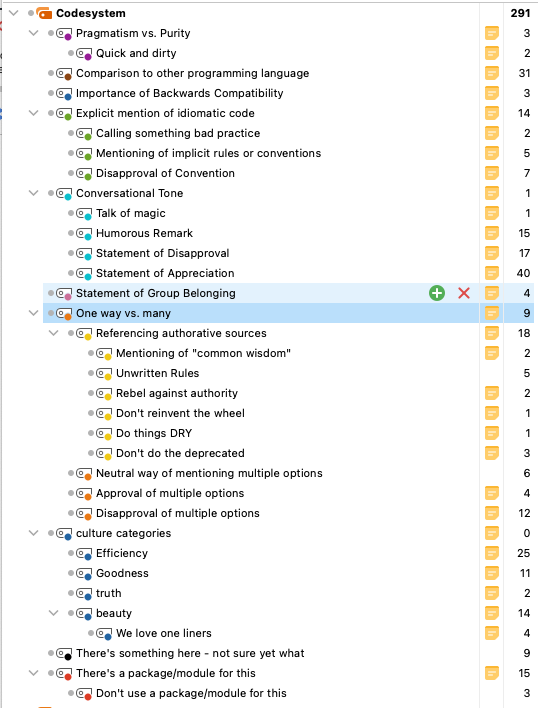
\includegraphics[width=0.7\textwidth]{early_code_system.png}


\end{document}
